
\chapter{Mail sending system}

Two kind of mail can be sent in \tria :
%Un module du programme permet d'envoyer des mails au créateur de l'ensemble des schémas et au développeurs de l'application. Deux types de mails peuvent être envoyés :\\
\begin{itemize}
\item A request to add a new relation.\\
%\item Une demande d'ajout d'une nouvelle relation. 
\item A report when an error has been met.\\
%\item Un rapport lorsqu'une erreur est survenue dans le logiciel. 
\end{itemize}

\section{Relation adding request}
In certain situations, it possible that the user do not find the real relation he needs. The objective "Other" is the first solutions to this kind of problem. But if the same relations is often needed, it possible to ask the schemes creator to add the relations to the lists of possibility in the next update.\\
%Dans certains, il est possible que l'utilisateur ne trouve pas de relation réelle convenant à la situation qu'il rencontre. L'objectif "Autre" permet de répondre à ce problème. Cependant, si une même relation manque à de nombreuses reprises, il est intéressant d'en informer le créateur de l'ensemble de schémas afin qu'il l'intègre à une futur version.\\

To do so, just lick on the option "Relation adding request" in the menu "Help".\\
%Pour réaliser cette demande, il suffit de cliquer sur l'option "Demande d'ajout de relation" dans le menu "Aide". Une fenêtre s'ouvre alors.\\


%L'adresse de réponse permet au destinataire de vous répondre directement.\\

%Les deux champs suivants correspondent au sujet et au contenu du mail envoyé.\\


\begin{figure}
\centering
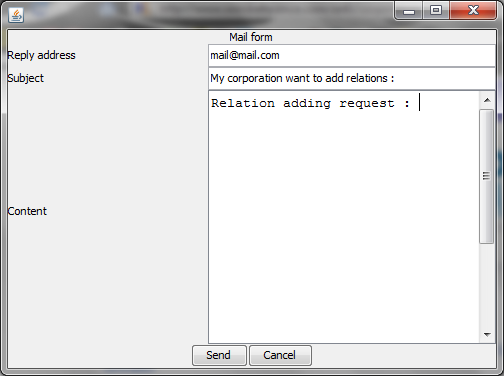
\includegraphics[width=12cm]{images/mail_relation.png}
\caption{The relation adding request window.}
\end{figure}


\section{Error report}

In despite of all the test realized in order to distribute a software of quality, it is still possible than some errors exist. If an error occurs, a pop-up will show and ask the user to send an error report. If this error is met for the first time, it is important to send this report with a description as precise as possible of the context of the error.\\ 
%Malgré l'ensemble des tests réalisés sur le logiciel \tria, il est possible qu'il subsiste quelques problèmes. Dans le cas où une erreur est rencontré, le logiciel vous propose automatiquement d'envoyer un mail aux développeurs. Cela leur permet d'identifier l'erreur et de la corriger par la suite.\\

%Il est très important de décrire l'action que vous étiez en train de réalisez lorsque l'erreur s'est produite. Cette description est une information souvent indispensable à la résolution du problème. Un texte généré automatiquement à l'intention des développeurs est ajouté à la fin du mail.\\

%Une boite de dialogue informe l'utilisateur qu'il est plus prudent de quitter l'application. Si c'est une erreur encore inconnue, il est fortement conseillé de quitter l'application. Dans le cas d'une erreur bénigne, les développeurs informeront l'utilisateur qu'il peut tout de même continuer à travailler (en répondant par mail à l'envoi du rapport d'erreur).\\





